%==============================================================================
\chapter{Introdução}\label{introducao}
%==============================================================================

O ato de classificar uma palavra pertencente a um conjunto de textos em uma classe gramatical depende de sua estrutura morfo-sintática, esse ato é conhecido no campo de \ac{pln} como \ac{pos} Tagging. A \autoref{fig:exemploclassificacao} ilustra esse processo. 

O conjunto de textos denominados \textit{córpus} são amplamente utilizados para esse processo, e é sobre eles que é feito o treinamento do modelo de reconhecimento de padrões para que seja possível classificar uma palavra a uma certa classe gramatical.

Um dos problemas dessa classificação é justamente a eficiência com o qual cada classe gramatical é atribuída para certa palavra, nesse quesito, há vários métodos já idealizados que conseguiram uma eficiência de cerca de 97\% \cite{dos2014training, collobert2011deep, fonseca2015evaluating}. \citeonline{fonseca2015evaluating} afirmam ter conseguido o estado-da-arte atual para o português com 97,57\% de acurácia.

Apesar de muitos desses métodos já serem utilizados em larga escala, em \ac{pln} estamos sempre buscando ganhar mais performance, já que \ac{pos} Tagging pode ser aplicada em uma grande variedade de aplicações como tradução automática e extração de informações de textos \cite{manning1999foundations}, ferramentas de auxílio à leitura e escrita \cite{marquiafavel2010processo}, entre outras.

\begin{figure}[htb]
  \caption{Exemplo de classificação gramatical}\label{fig:exemploclassificacao}
  \begin{center}
      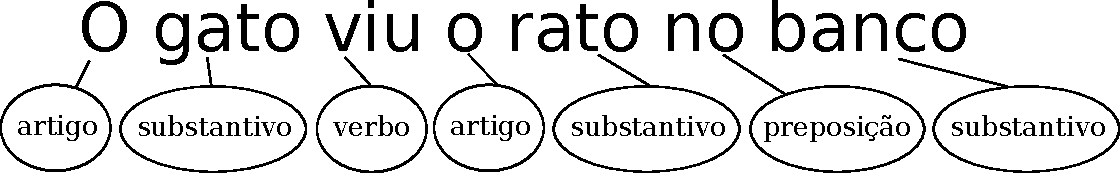
\includegraphics[scale=0.75]{img/exemploclassificacao.pdf}
  \end{center}
\end{figure}

Nosso trabalho consiste em classificar palavras de acordo com seu contexto, ou seja, é feita a análise em termos das unidades primitivas que a compõem, e uma vez que ela é cumprida, podemos aplicar o resultado em outras análises.


%------------------------------------------------------------------------------
\section{Objetivo}\label{sec:objetivo}
%------------------------------------------------------------------------------

Este trabalho tem, por fim, propor um novo método de classificação de palavras em classes gramáticais e analisar sua eficiência em relação a trabalhos já publicados que utilizam métodos já consolidados. Primordialmente, isso será feito para o escopo da língua portuguesa brasileira. 

Para buscar uma boa eficiência será proposto um método original, que se baseia em classificar primeiramente palavras mais fáceis (\textit{e.g verbos}), desse modo, espera-se deixar palavras ambíguas por último. Por exemplo, para a \autoref{fig:exemploclassificacao} deixaríamos a palavra \textit{canto} para o final, uma vez que não sabemos se isso se trata de um verbo ou de um substantivo.  

Como já mencionado, o estado-da-arte atual tem atualmente cerca de 97\% de acurácia, tentaremos ultrapassar esse limite aplicando novas técnicas de classificação e utilizando características significantes das palavras. A acurácia da classificação não será a única medida levada em consideração, o tempo de processamento gasto no treinamento para cada \textit{córpus} também será.

Para exemplificar brevemente uma possível aplicação, no final pretende-se que o modelo seja capaz de classificar corretamente as palavras analisando o seu contexto, e com isso outros analisadores conseguirão identificar o uso das palavras de acordo com seu significado, como mostrado abaixo na \autoref{eq:exemploobjetivo}. Essa equação será explicada na \autoref{sec:representacaodaspalavras}.

\begin{equation}
\texttt{homem + coroa = rei} \label{eq:exemploobjetivo}
\end{equation}



%------------------------------------------------------------------------------
\section{Estrutura do trabalho}\label{sec:estruturadotrabalho}
%------------------------------------------------------------------------------

A fim de proporcionar uma boa interpretação, este trabalho foi dividido nos seguintes capítulos: No \autoref{oproblema} será descrito o problema de etiquetagem. No \autoref{fundamentos} será mostrados os principais fundamentos necessários para entender o método proposto e seus conceitos relacionados; após passar os fundamentos, será apresentado no \autoref{trabalhosrelacionados} os trabalhos relacionados que procuram resolver o problema de \ac{pos} Tagging utilizando diferentes técnicas e abordagens. Depois, no \autoref{desenvolvimento} será detalhado aspectos da metodologia a ser aplicada e a explicação do método proposto juntamente com as técnicas utilizadas. Então, no \autoref{comparativo} será feito um comparativo entre os resultados preliminares alcançados e uma breve discussão a respeito. E por fim, no \autoref{conclusao} será apresentado as considerações finais.
